\chapter{Návrh funkcí a architektury reálné aplikace}

Po dokončení návrhu GUI, popisovaného v předchozí kapitole, bylo ještě před započetím implementace potřeba rozhodnout o několika pokročilých funkcích, které vyžadují spolupráci frontendu s backendem. Kromě toho bylo také nutné dokončit soupis procesů pro roli vedoucího skladu, neboť ten byl v rámci MI-NUR přeskočen, zvolit použitou technologii a vybrat barevnou paletu aplikace - všechny tyto body budu diskutovat na následujících řádcích.

\section{Návrh pokročilých funkčností aplikace}

V této sekci budu diskutovat funkce, které byly analyzovány ještě před započením implementace samotné aplikace a jejíchž analýze byl věnován určitý nezanedbatelný čas.

%%%%%%%%%%%%%%%%%%%%%%%%%%%%%%%%%%%%%%%%
%%%%%%%%%%%%%%%%%%%%%%%%%%%%%%%%%%%%%%%%

\subsection{Undo}\label{draft:undo}

Undo, neboli možnost vrácení akce, tlačítko \emph{zpět}, \emph{vrátit} či \emph{stornovat}. Tím vším je myšlena možnost odvrátit poslední akci, kterou uživatel v systému provedl. Undo je svým způsobem alternativa potvrzovacím dialogům, u kterých bych se chtěl ještě na chvilku zastavit.

\paragraph{Potvrzovací dialogy} Všichni je známe - modální okna, typicky s otázkou a dvěma akcemi: \emph{opravdu smazat/odeslat/\ldots} a \emph{storno}. Jsou používány tam, kde jejích potvrzení je většinou nevratné a dojde k provedení něčeho důležitého. Co když je ale provádění důležitých akcí stěžejní funkčností systému? V příkladu skladového systému jsou veškeré přesuny zboží, naskladnění, vyskladnění atp. důležité akce, u kterých by si měl skladník zkontrolovat, že realita odpovídá stavu v systému. Potvrzovací dialogy na všech těchto akcích ale mohou uživatele i zdržovat - akce, která je v systému vykonávána s vysokou frekvencí, by neměla stále dokola vyžadovat dvojité potvrzení. Nejen že to bude uživatele zdržovat, ale i samotná četnost zapříčiní, že potvrzovací dialog ztratí svůj účel - uživatel bude zvyklý jej \emph{ihned odkliknout}, aniž by se zamyslel nad tím, zda akci chce opravdu provést \cite{nn-dialogs}. 

\paragraph{Undo} Možnost vrátit akci zpět je svým způsobem volnější než potvrzovací dialog - nezdržuje dvojitým potvrzením, ale v případě nutnosti umožňuje špatné rozhodnutí vrátit. Většinou ale nedává moc času na rozmyšlenou - možnost vrátit akci se typicky zobrazuje pouze několik sekund. Také implementace je často mnohem složitější a vyžaduje řádný návrh a spolupráci prezenční a modelové či datové vrstvy.

Při návrhu \emph{undo tlačítka} pro skladový systém jsme společně s Pavlem Kovářem\footnote{spoluautor návrhového řešení - zabývá se backendovou částí aplikace} zanalyzovali několik možností:
\begin{enumerate}
	\item \textbf{Fronta ve frontendu:} Frontendu by při provedení akce, která by podporovala undo, požadavek reálně neodeslal, ale uložil by jej k pozdějšímu odeslání - například za 5 sekund. Při kliku na undo by se odložené odeslání akce stornovalo, v opačném případě by se požadavek odeslal buďto po uplynutí stanového doby, nebo před provedením jiné další akce.\\\\
	\emph{Zhodnocení řešení:} Jedná se o nejsnadnější implementaci - nevyžaduje žádné úpravy backendu a vše se řeší pouze na klientských zařízeních. S tím ale přichází i hlavní nedostatky tohoto řešení: Když klient ukončí či ztratí spojení se serverem, požadavek se reálně neodešle, přestože systém hlásí, že je odeslaný. Dále když jiný klient provede stejnou akci, dorazí pak na server obě a druhá nemůže být provedena - je potřeba o tom uživatele informovat a problém řešit. Oba problémy jsou poměrně zásadní, a tak byla tato varianta provedení zavržena.
	\item \textbf{Fronta jako middleware:} Frontend by odesílal požadavky ihned, avšak mezi ním a backendem by existoval ještě prostředník: fronta ke zpracování. Ta by požadavky zachytávala a čekala s jejich reálným odesláním backendu. Chování by bylo podobné, jako kdyby s odesláním čekal frontend v předchozí variantě.\\\\
	\emph{Zhodnocení řešení:} Jedná se o řešením, jak předcházet problémům s potenciální ztrátou připojení. Middleware by sloužil jako fronta pro všechny klienty serveru. Když pak klient ztratí či ukončí připojení, požadavek se provede, neboť middleware jej na backend odešle sám. Při ztrátě připojení by se uživateli, který by chtěl použít undo zobrazí informace o ztrátě připojení a informace, že požadavek již byl proveden a bohužel nemůže být stornován.\\
	I zde ale přetrvává problém se synchronizací mezi více klienty - frontend by musel pro každý požadavek, který šel přes frontu, zpětně kontrolovat, že byl nakonec vykonán bezchybně a případně informovat uživatele. To je nepohodlné, ale na druhou stranu ne zcela nereálné řešení.
	\item \textbf{Fronta v backendu:} Požadavky by se odesílaly na backend ihned, a ten by si sám držel frontu obdržených požadavků, ke kterým ještě může přijít požadavek na undo. Opět po uplynutí doby, nebo přijetí požadavku na potvrzení by se změny reálně provedly a potvrdily.\\\\
	\emph{Zhodnocení řešení:} Třetí řešení je velmi podobné tomu druhému, změnou je, že když si bude frontu udržovat přímo backend, může ten s čekajícími požadavky již počítat při vracení dat jiným klientům (soft lock) - a tím předcházet nekonzistencím v datech: Když uživatel A vyskladní poslední kus výrobku, ale tento požadavek ještě čeká ve frontě, uživateli B se již bude zobrazovat, že je na skladě 0 kusů tohoto výrobků a nemůže ho tak vyskladnit duplicitně.\\
	Problémem tohoto řešení je velmi velká náročnost na zpracování těchto zámků a poměrně vysoká šance na neúmyslné chyby v kódu. Z toho důvodu jsme nakonec tuto variantu také zavrhli.
	\item \textbf{Změnové vektory v backendu:} Frontend by vše odesílal hned, backend by vše ihned zpracovával. Kromě zpracování by ale ukládal i změnové vektory, které by bylo možné zpětně odvolat - provést \emph{rollback}. Změnové vektory jsou technikou často používanou například v databázových strojích - veškeré změny jsou zaznamenávány a posléze je možné vše zpětně přehrát a vrátit tak předchozí stav \cite{valenta-db}.\\\\
	\emph{Zhodnocení řešení:} V běžné implementaci tato technika umožňuje navrátit stav \emph{celé databáze}, nikoliv pouze jednoho uživatele. Pokud by tedy chtěl undo použít pouze jeden klient, vrátil by se stav i ostatním uživatelům, které si undo vůbec nepřejí. Pro potřeby undo jednoho klienta by tak musely být provedeny mnohé úpravy, a ty by byly neúměrně náročné vůči výsledku. Z důvodu robustnosti tedy tuto variantu taktéž zavrhujeme.
	\item \textbf{Přímá podpora undo v API:} Backendové metody by nativně podporovaly možnost zavolat na určité akce undo: u vybraných funkcí by byla příbuzná metoda, která by jako parametr přijímala identifikátor zaslaný jako výsledek předchozí akce. Jednotlivé požadavky by tak nebyly nijak zdržovány a vše by se provádělo ihned, a požadavek na vrácení změn by byl zpracován jako zcela nová akce.\\\\
	\emph{Zhodnocení řešení:} Mezi výhody posledního z návrhů patří zejména to, že při něm není potřeba řešit konzistenci dat mezi více klienty, vše je ihned potvrzeno a změny se řeší nezávisle na předchozím požadavku. Nevýhodou je, že to není obecné řešení - je potřeba tyto metody implementovat pro všechny akce, které mají undo podporovat. Opět se ale jedná o reálně použitelné řešení, které bude implementováno pouze tam, kde to dává smysl.
\end{enumerate}

Po zhodnocení všech variant jsem se rozhodli jít prozatím cestou pátého návrhu - přímé podpory pouze u vybraných akcí. Důvodem je i fakt, že ve většině akcí by v systému ani chybu jít udělat \emph{nemělo} - tím jsme se posunuli od potvrzovacího dialogu, přes undo, až po \emph{prevenci chyb}. Například u vyskladnění vidí skladník jasný seznam položek, které má vyskladnit, a pokud nemá vše \emph{napípáno}, systému mu ani úkol dokončit nedovolí. U některých vybraných akcí půjde undo provést, a u zbylých, které vyhodnotím jako důležité a málo časté, kde nepůjde realizovat ani prevence chyb, ani undo, skončím u běžných potvrzovacích dialogů.\\
Realizace tohoto návrhu je popsána v sekci \ref{implementation:undo}.

%%%%%%%%%%%%%%%%%%%%%%%%%%%%%%%%%%%%%%%%
%%%%%%%%%%%%%%%%%%%%%%%%%%%%%%%%%%%%%%%%

\subsection{Zkratky v systému za použití čtečky čárových kódů}

Nápad na tuto funkci vychází z faktu, že drtivá většina skladníků, kteří budou se systémem pracovat, budou mít v ruce zařízení podporující skenování položek a okamžité předávání načteného kódu přímo do aplikace.\\
Návrhem k realizaci tedy je, že by skladník nemusel načítat pouze EANy položek a čárové kódy umístění, ale mohl by přes čtečku iniciovat i určité akce - například v místě, kde přechází k přebírání dorazivších dodávek zboží by mohl být nalepen kód, který v aplikaci spustí úlohu \emph{Příjem dodávky}. V místě, kde se vyzvedávají palety, vozíky či cokoliv jiného, co čeho se kompletuje vyskladnění, by zase mohl být kód pro iniciování úlohy vyskladnění - a pokud by vyskladnění nemohl iniciovat skladník sám, tak by se například mohl otevřít seznam vyskladnění, která čekají na vyřízení.\\
Konkrétní seznam kódů a akcí, které se mají stát, by ideálně měl být konfigurovatelný přímo ze systému, aby byl skladový systém použitelný pro různé typy skladů.


\section{Návrh procesů v novém skladovém systému}

Před započetím samotné implementace bylo nutné dokončit návrh procesů v systému, za jejímž účelem vznikl dokument popisující procesy rolí skladníka a vedoucího skladu.\\
Dokument je rozdělen na následující části:
\begin{enumerate}
	\item Slovník pojmů,
	\item entity a jejich atributy z pohledu uživatele,
	\item procesy shodné pro obě role,
	\item procesy role \emph{skladník},
	\item procesy role \emph{vedoucí},
	\item angler (autorizační server).
\end{enumerate}
Z důvodu, že má dokument deset stran a obsahuje formátování napomáhající porozumění, ho nebudu vkládat přímo do textu, ale je možné jej nalézt jako přílohu \ref{ap:processes} nebo v souboru \code{processes.pdf} na přiloženém médiu.


\section{Volba technologie}\label{technology}

Jelikož bude aplikace rozdělena na backend, kterým se zabývá můj kolega Bc.~Pavel Kovář, a frontend, který je předmětem této práce, je žádoucí věnovat jistou část textu volbě vhodné technologie.

\paragraph{Cílová platforma} Aplikace je navrhována s ohledem na hardwarové vybavení skladu, ve kterém bude poprvé nasazována: zdejší skladníci jsou vybaveni mobilními telefony \emph{Zebra TC25BJ}, které disponují OS Android 7.1 a vestavěnou čtečkou čárových kódů. Kromě skladníků by měla být aplikace použitelná také z tabletu či stolního počítače pro účely vedoucích pracovníků. Z důvodu jednoduchosti vývoje,  testování, možností aktualizací a obecně dobré zkušenosti z jiných projektů bylo hned při úvodním návrhu určeno, že aplikace bude tvořena formou webové služby, která bude na klientských zařízeních zobrazována ve WebView v jednoduchém kontejneru chovajícím se jako nativní aplikace. Řídící pracovníci budou naopak moci využít přístupu odkudkoliv, kde budou připojeni k internetu pouze pomocí běžného webového prohlížeče.\\
Z tohoto důvodu jsou v následující rešerši zhodnocovány frameworky či knihovny, které usnadňují vývoj \emph{webových aplikací}.

\paragraph{Frameworky a knihovny} V době psaní této práce patří mezi nejpopulárnější \cite{frameworks-github} \cite{frameworks-hackr} front-endové frameworky či knihovny Angular \cite{angular}, React \cite{react}, Vue.js \cite{vue}, Ember.js \cite{ember} a Backbone.js \cite{backbone}.

\paragraph{Názvosloví} Pro účely tohoto textu budu na následujících řádcích používat slovo \emph{framework}, kterým budu označovat jak frameworky, tak knihovny, z důvodu snížení opakování textu.\\

%%%%%%%%%%%%%%%%%%%%%%%%%%%%%%%%%%%%%%%%
%%%%%%%%%%%%%%%%%%%%%%%%%%%%%%%%%%%%%%%%

\subsection{Datum vydání}

Zatímco v současnosti nejčastěji porovnávanými frameworky jsou první dva zmíněné, Vue.js je z této pětice vybraných nejmladší, nabírá ale velké obliby. Ember.js a Backbone.js jsou poté lehce upozaděny z důvodu jejich stáří. Přehled prvního vydání jednotlivých frameworků je v tabulce \ref{table:compare:release}

\begin{table}[h]
\caption{Volba frameworku: Datum vydání}
\label{table:compare:release}
\begin{tabular}{lrrrrr}
\hline
                                         & Angular                     & React                     & Vue.js                     & Ember.js                     & Backbone.js               \\ \hline
Vydání první verze                       & 2010/2016\footnote{\ V roce 2010 byl vydán AngularJS, který byl v roce 2016 kompletně přepsán do TypeScriptu a vydán jako Angular 2, či jednoduše \emph{Angular}.}                                                                       & 2013                      & 2014                       & 2011                         & 2010                      \\
\end{tabular}
\end{table}

Datum vydání ovšem nelze objektivně ohodnotit bodovým ziskem. Na jedné straně stojí fakt, že starší framework může být vyspělejší a tudíž stabilnější atp., na straně druhé nové frameworky se často učí z chyb provedených jejich předchůdci a vyberou z nich pouze to nejlepší. Tato tabulka tedy zůstane čistě přehledová.

%%%%%%%%%%%%%%%%%%%%%%%%%%%%%%%%%%%%%%%%
%%%%%%%%%%%%%%%%%%%%%%%%%%%%%%%%%%%%%%%%

\subsection{Zázemí}

Zatímco Angular a React jsou vyvíjeny velkými společnostmi: Googlem, respektive Facebookem, které zná každý, Ember.js je vyvíjen společností Tilde Inc. \cite{tilde}, která také není žádným startupem. Vue.js a Backbone.js by se naopak daly nazvat \emph{komunitními projekty}, neboť jsou vytvořeny převážně jedním autorem (Evan You, respektive Jeremy Ashkenas) a rozvíjeny a udržovány komunitou vývojářů. 
\\
Na první pohled by se mohlo zdát, že z tohoto hodnocení budou vycházet lépe ty frameworky, které mají za sebou stabilní firmy, neboť je tím zajištěn jejich kontinuální vývoj. Ve skutečnosti ale velké firmy \emph{zabíjejí} své projekty poměrně často, stačí se podívat například na seznam projektů, které ukončil Google \cite{killed_by_google}. Oproti tomu komunitní projekty mohou žít dále i v případě, že jejich hlavní autor už na projektu nechce, nebo nemůže pracovat. Z toho důvodu nelze jednoznačně určit, které zázemí je pro budoucnost frameworku výhodnější, a u tabulky \ref{table:compare:background} se tedy opět zdržuji udělování bodů.

\begin{table}[h]
\caption{Volba frameworku: Zázemí}
\label{table:compare:background}
\begin{tabular}{lrrrrr}
\hline
                                         & Angular                     & React                     & Vue.js                     & Ember.js                     & Backbone.js               \\ \hline
Zázemí velké\\společnosti                & ano                         & ano                       & ne                         & částečně                     & ne                        \\
\end{tabular}
\end{table}

%%%%%%%%%%%%%%%%%%%%%%%%%%%%%%%%%%%%%%%%
%%%%%%%%%%%%%%%%%%%%%%%%%%%%%%%%%%%%%%%%

\subsection{Licence}

Licence k použití frameworku je důležitá položka při rozhodování. Naštěstí všech 5 porovnávaných frameworků je v době psaní této licencováno pod MIT licencí, která povoluje jakékoliv použití i v komerční sféře, úpravy, distribuce i použití v ne-opensource projektech. Nevýhodou této licence je nulová záruka funkčnosti či zodpovědnost autorů za potenciální spáchané škody tímto softwarem.
\\
\paragraph{Licencování Reactu} Facebook původně vydal svůj React pod BSD licencí spolu s dalšími patenty, avšak 24. září 2017 byl React převeden pod MIT licenci \cite{react-license-commit, react-license}.
\\
Jelikož jsou všechny frameworky licencovány stejně, neprobíhá v tabulce \ref{table:compare:license} žádné bodování.

\begin{table}[h]
\caption{Volba frameworku: Licence}
\label{table:compare:license}
\begin{tabular}{lrrrrr}
\hline
                                         & Angular                     & React                     & Vue.js                     & Ember.js                     & Backbone.js               \\ \hline
Licence                                  & MIT                         & MIT                       & MIT                        & MIT                          & MIT                       \\
\end{tabular}
\end{table}

%%%%%%%%%%%%%%%%%%%%%%%%%%%%%%%%%%%%%%%%
%%%%%%%%%%%%%%%%%%%%%%%%%%%%%%%%%%%%%%%%

\subsection{Křivka učení}

Složitost frameworku je důležitá metrika, neboť má dopady zejména na ekonomickou stránku projektu. Jednoduché prvotní vniknutí do problematiky frameworku ovšem také nemusí být nutně výhodou, pokud v něm je později problémové provést některé pokročilé věci, nebo i v pokročilém stádiu zdržuje svým nízkoúrovňovým přístupem k problémům, které jiné frameworky řeší automaticky.

\paragraph{Angular, React a Vue.js} Přehled obtížnosti tří v současnosti nejčastěji skloňovaných frameworků přehledně shrnul Rajdeep Chandra ve své prezentaci \emph{My experience with Angular 2 , React and Vue} \cite{frameworks-3compare}, ze které vychází hodnocení v tabulce \ref{table:compare:difficulty}.

\paragraph{Ember.js} Tento framework je dle V. Lascika \cite{ember-diffuculty} vhodný spíše pro projekty, na kterých pracuje velké množství vývojářů, a to z důvodu své komplexnosti. Proto jej pro použití v mé vznikající aplikaci hodnotím nula body.

\paragraph{Backbone.js} U této knihovny je důležité zmínit, že umožňuje vývojáři vytvořit si strukturu aplikace kompletně dle svého uvážení \cite{frameworks-rubygarage}. To ssebou může nést jak výhody pro zkušeného, tak nevýhody pro nezkušeného vývojáře, který v pokročilém stádiu vývoje může zjistit, že některou ze základních struktur navrhl špatně. Samotná obtížnost práce s touto knihovnou je ale poměrně nízká.

\begin{table}[h]
\caption{Volba frameworku: Obtížnost}
\label{table:compare:difficulty}
\begin{tabular}{lrrrrr}
\hline
                                         & Angular                     & React                     & Vue.js                     & Ember.js                     & Backbone.js               \\ \hline
Obtížnost                                & vysoká                      & vyšší                     & nízká                      & velmi vysoká\footnote{\ za předpokladu, že na projektu bude pracovat pouze velmi malé množství vývojářů}                                                                                                                                & nízká                     \\
\makecell[r]{\textit{bodový zisk}}       & \textit{1}                  & \textit{2}                & \textit{4}                 & \textit{1}                   & \textit{4}                  
\end{tabular}
\end{table}

%%%%%%%%%%%%%%%%%%%%%%%%%%%%%%%%%%%%%%%%
%%%%%%%%%%%%%%%%%%%%%%%%%%%%%%%%%%%%%%%%

\subsection{Oficiální dokumentace}

Hlavním zdrojem ke studiu frameworku by měla být jeho oficiální dokumentace, v této sekci tedy budu hodnotit kvalitu a obsáhlost oficiálního manuálu k jednotlivým frameworkům.

\paragraph{Angular} Jedná se o velmi obsáhlou a dobře rozdělenou dokumentaci \cite{angular-doc}, která obsahuje i řadu příkladů a ve srozumitelné stromové struktuře vývojář jednoduše najde, co potřebuje.

\paragraph{React} Dokumentace Reactu \cite{react-doc} je o poznání jednodušší než ta Angularu, avšak to je způsobeno tím, že React je pouze knihovna, kdežto Angular je plnohodnotný framework. Dokumentace je rozdělena na jednodušší úvod a pokročilejší techniky, je tedy snadné s ní pracovat.

\paragraph{Vue.js} Nejmladší z frameworků má také velmi přátelskou dokumentaci \cite{vue-doc}, která je podobně jako u Angularu velmi bohatá a stromově strukturovaná.

\paragraph{Ember.js} Oficiální manuál Ember.js \cite{ember-doc} je taktéž poměrně obsáhlý a strukturou připomíná dokumentaci Angularu a Vue.js. Obsahuje velké množství ukázek kódu a je logicky strukturován.

\paragraph{Backbone.js} Poslední ze zkoumaných frameworků má oficiální dokumentaci \cite{backbone-doc} na první pohled méně atraktivní a pro nováčka může být matoucí. Oproti ostatním dokumentacím chybí například barevné zvýraznění důležitých bodů a další grafické strukturování textu.

\begin{table}[h]
\caption{Volba frameworku: Dokumentace}
\label{table:compare:docs}
\begin{tabular}{lrrrrr}
\hline
                                         & Angular                     & React                     & Vue.js                     & Ember.js                     & Backbone.js               \\ \hline
\makecell{Kvalita oficiální\\dokumentace} & \makecell{velmi\\vysoká}   & vysoká                    & \makecell{velmi\\vysoká}   & \makecell{velmi\\vysoká}     & střední                   \\
\makecell[r]{\textit{bodový zisk}}       & \textit{3}                  & \textit{2}                & \textit{3}                 & \textit{3}                   & \textit{1}                  
\end{tabular}
\end{table}

%%%%%%%%%%%%%%%%%%%%%%%%%%%%%%%%%%%%%%%%
%%%%%%%%%%%%%%%%%%%%%%%%%%%%%%%%%%%%%%%%

\subsection{Testování}

Testování je při vývoji softwaru velkým tématem. Mnoho vývojářů nerado testuje, jiní se naopak specializují pouze na testování. V moderních aplikacích je testování z větší části řešeno automatizovanými testy, které se spouští v rámci CI. Přestože se tato práce zabývá pouze frontendem, i ten je možné testovat již od úrovně Unit testů, vyvíjej jej pomocí TDD a nakonec samozřejmě vše zkontrolovat pomocí E2E testů.

\paragraph{Angular} Nejkomplexější z frameworků nabízí přehlednou dokumentaci \cite{angular-test}, jak by měl být testován. Popisuje jak používat Unit testy i E2E testy a pro druhý zmíněný typ nabízí i samotný testovací framework: Protractor \cite{protractor}. Jeho testovatelnost tedy hodnotím jako velmi dobrou.

\paragraph{React} Tato knihovna ve své dokumentaci na první pohled testování příliš neprosazuje, avšak stránku dedikovanou této kratochvíli \cite{react-test} lze nakonec také nalézt. Narozdíl od Angularu zde není poskytován dedikovaný framework určený přímo pro testování této knihovny. Stránka popisuje testovací frameworky, které používají různé společnosti: autoři Reactu - Facebook - zmiňují svůj Jest \cite{jest}, také je ale zmiňován Enzyme \cite{enzyme} od Airbnb. Konkrétní příklady použití bychom tedy dále hledali v dokumentacích těchto frameworků. Celkově je pro React k dispozici více různých testovacích frameworků, které opět pokrývají jak Unit, tak E2E testování.

\paragraph{Vue.js} Ani Vue.js se neztratí co se Unit a E2E testů týká. Přímo ve své dokumentaci \cite{vue-test} popisuje spouštění Unit testů pomoci vestavěných příkazů, které interně používají buďto již zmiňovaný Jest nebo Mocha \cite{mocha}, a dále odkazuje na vlastní kompletní testovací knihovnu \cite{vue-test-utils}. Také je možné použít velké množství různých testových frameworků a aplikace ve Vue.js lze vyvíjet i pomocí TDD \cite{vue-tdd}.

\paragraph{Ember.js} Tento framework se ve své dokumentaci věnuje testování poměrně intenzivně a zasvětil mu rovnou několik stránek \cite{ember-test}. Jako výchozí testovací framework představuje vlastní QUnit, avšak informuje, že je možné použít i frameworky třetích stran. Testování přehledně rozděluje na \emph{Unit}, \emph{Container}, \emph{Render}, a \emph{Application} testy a také popisuje jak testovat jednotlivé komponenty. Testování Ember.js tedy také hodnotím jako velmi dobré.

\paragraph{Backbone.js} U posledního zkoumaného frameworku na první pohled není testování moc jasné. Oficiální stránka odkazuje na \emph{test suite} \cite{backbone-test}, což je ovšem stránka, která testy \emph{spouští} a ne popisuje. Zdá se, že na této stránce je možné otestovat svůj prohlížeč, zda podporuje veškeré funkcionality Backbone.js. Co se psaní testů týká, rozumněji již vypadá externí stránka \emph{Backbone.js Testing} \cite{backbone-testing}, která již zmiňuje i zde dříve probírané frameworky jako \emph{Mocha}. Ve výsledku tak bude pravděpodobně testování Backbone vypadat obdobně jako u ostatních frameworků, avšak přístup oficiální dokumentace snižuje jeho pochopení.

\begin{table}[h]
\caption{Volba frameworku: Testování}
\label{table:compare:tests}
\begin{tabular}{lrrrrr}
\hline
                                         & Angular                     & React                     & Vue.js                     & Ember.js                     & Backbone.js               \\ \hline
\makecell[l]{Možnosti testování\\a jejich popis\\v dokumentaci} &\makecell[l]{velmi\\kvalitní} &\makecell[l]{velmi\\kvalitní} &\makecell[l]{velmi\\kvalitní} &\makecell[l]{velmi\\kvalitní} &matoucí \\
\makecell[r]{\textit{bodový zisk}}       & \textit{2}                  & \textit{2}                & \textit{2}                 & \textit{2}                   & \textit{1}                  
\end{tabular}
\end{table}

%%%%%%%%%%%%%%%%%%%%%%%%%%%%%%%%%%%%%%%%
%%%%%%%%%%%%%%%%%%%%%%%%%%%%%%%%%%%%%%%%

\subsection{Vývojářské nástroje}

Dalším důležitým nástrojem při práci s frameworkem je možnost jeho debuggování. Framework by měl nabízet vlastní řešení, které vývojáři usnadní nalézt chybu, zjistit, jak se jeho kód chová či odladil rychlostní problémy.
\\
Všechny ze zde porovnávaných frameworků nabízejí tyto nástroje formou doplňku do prohlížeče, konkrétně se dále budeme bavit o doplňcích pro Google Chrome.

\begin{table}[h]
\caption{Volba frameworku: Devtools}
\label{table:compare:devtools}
\begin{tabular}{lrrrrr}
\hline
                                         & Angular                     & React                     & Vue.js                     & Ember.js                     & Backbone.js               \\ \hline
Název                                    & Augury    & \makecell[r]{React\\Developer\\Tools} & \makecell[r]{Vue.js\\devtools} & \makecell[r]{Ember\\inspector} & \makecell[r]{Backbone\\Debugger} \\
Počet stažení\footnote{\ Stav k 24. 12. 2018}  & 230k                    & 1.351k                    & 706k                       & 57k                          & 9,5k                      \\
\makecell[r]{\textit{bodový zisk}}       & \textit{2}                  & \textit{4}                & \textit{3}                 & \textit{1}                   & \textit{0}                \\
Hodnocení (z 5)                          & 3.9                         & 4.2                       & 4.7                        & 4.8                          & 4.5                       \\
\makecell[r]{\textit{bodový zisk}}       & \textit{1}                  & \textit{2}                & \textit{3}                 & \textit{3}                   & \textit{3}                  
\end{tabular}
\end{table}

%%%%%%%%%%%%%%%%%%%%%%%%%%%%%%%%%%%%%%%%
%%%%%%%%%%%%%%%%%%%%%%%%%%%%%%%%%%%%%%%%

\subsection{Počet hvězdiček na GitHubu}

Počet hvězdiček na GitHubu lze velmi volně interpretovat jako oblíbenost frameworku mezi vývojáři. Z tohoto důvodu již v tabulce \ref{table:compare:github_stars} hodnotím frameworky dle počtu získaných hvězdiček.

\begin{table}[H]
\caption{Volba frameworku: Počet hvězdiček na GitHubu}
\label{table:compare:github_stars}
\begin{tabular}{lrrrrr}
\hline
                                         & Angular                     & React                     & Vue.js                     & Ember.js                     & Backbone.js               \\ \hline
Počet hvězdiček\\na GitHubu\footnote{\ Stav k 17. 12. 2018} &   43,6k    & 117,7k                    & 122,3k                     & 20,3k                        & 27,3k                     \\
\makecell[r]{\textit{bodový zisk}\footnote{\ Hodnocení přeskakuje bodový zisk 3, aby bylo zhodnoceno i absolutní množství hvězdiček, nejen pořadí.}}
                                         & \textit{2}                  & \textit{4}                & \textit{5}                 & \textit{0}                   & \textit{1}                  
\end{tabular}
\end{table}

%%%%%%%%%%%%%%%%%%%%%%%%%%%%%%%%%%%%%%%%
%%%%%%%%%%%%%%%%%%%%%%%%%%%%%%%%%%%%%%%%

\subsection{Počet npm balíků}

Npm \cite{npm} je repozitář javascriptových komponent, na kterém jsou sdíleny jednak kompletní řešení (jako například Angular, Rect, Vue.js a další), ale především různé rozšiřující pluginy do těchto frameworků. Z toho důvodu budu v následující metrice hodnotit, kolik balíků npm nabízí pro jednotlivé porovnávané frameworky.
\\
Bodové zisky hrubě odpovídají relativnímu počtu nalezených balíků.

\begin{table}[h]
\caption{Volba frameworku: Počet npm balíků}
\label{table:compare:npm}
\begin{tabular}{lrrrrr}
\hline
                                         & Angular                     & React                     & Vue.js                     & Ember.js                     & Backbone.js               \\ \hline
Počet npm balíků                         & 26,6k                       & 73,4k                     & 20,6k                      & 6,4k                         & 1,5k                      \\
\makecell[r]{\textit{bodový zisk}}       & \textit{2}                  & \textit{3}                & \textit{2}                 & \textit{1}                   & \textit{0}                 
\end{tabular}
\end{table}

%%%%%%%%%%%%%%%%%%%%%%%%%%%%%%%%%%%%%%%%
%%%%%%%%%%%%%%%%%%%%%%%%%%%%%%%%%%%%%%%%

\subsection{Otázky na Stack Overflow}

Stack Overflow je jedním z portálů sítě Stack Exchange, který zná prakticky každý vývojář. Kdokoliv zde může položit otázku a komunita poté odpovídá, zatímco hlasuje o kvalitě odpovědí, aby byla vybrána ta nejlepší.\\
Z pohledu volby frameworku může být na jednu stranu vhodné, aby bylo na této stránce hodně otázek týkajících se dané technologie, na druhou stranu to ale může znamenat i nekvalitní dokumentaci. Jelikož ale v předchozí sekci nebyla žádná dokumentace vyhodnocena jako vysloveně špatná, budu dále usuzovat, že větší množství otázek je lepší.

\begin{table}[h]
\caption{Volba frameworku: Otázky na Stack Overflow}
\label{table:compare:stackoverflow}
\begin{tabular}{lrrrrr}
\hline
                                         & Angular                     & React                     & Vue.js                     & Ember.js                     & Backbone.js               \\ \hline
\makecell[l]{Počet otázek\\na Stack Overflow} & 146k                   & 118k                      & 28k                        & 23k                          & 21k                       \\
\makecell[l]{Počet \emph{zodpovězených}\\otázek} & 86k                 & 72k                       & 18k                        & 17k                          & 16k                       \\
\makecell[r]{\textit{bodový zisk}}       & \textit{3}                  & \textit{3}                & \textit{1}                 & \textit{1}                   & \textit{1}                  
\end{tabular}
\end{table}

%%%%%%%%%%%%%%%%%%%%%%%%%%%%%%%%%%%%%%%%
%%%%%%%%%%%%%%%%%%%%%%%%%%%%%%%%%%%%%%%%

\subsection{Firemní stack}

Další zvolenou metrikou je, jak daná technologie zapadá do firemní stacku firmy Jagu s.r.o., ve které bude tento nový projekt realizován. Firma se specializuje především na webové aplikace a middlewary na zakázku \cite{jaguweb}, a mezi nejpoužívanější technologie patří PHP (Nette, Laravel, Symfony), dále provozuje jeden informační systém postavený na Angularu a nově také menší aplikaci ve Vue.js. Tabulka \ref{table:compare:stack} shrnuje, jak jsou jednotlivé frameworky blízko k tomuto stacku.

\begin{table}[h]
\caption{Volba frameworku: Shoda s firemním stackem}
\label{table:compare:stack}
\begin{tabular}{lrrrrr}
\hline
                                          & Angular                     & React                     & Vue.js                     & Ember.js                     & Backbone.js               \\ \hline
Shoda s\\firemním stackem                 & ano                         & ne                        & ano                        & ne                           & ne                        \\
\makecell[r]{\textit{bodový zisk}}        & \textit{2}                  & \textit{0}                & \textit{2}                 & \textit{0}                   & \textit{0}                  
\end{tabular}
\end{table}

%%%%%%%%%%%%%%%%%%%%%%%%%%%%%%%%%%%%%%%%
%%%%%%%%%%%%%%%%%%%%%%%%%%%%%%%%%%%%%%%%

\subsection{Dostupnost vývojářů}

Metrikou, kterou z hlediska udržitelnosti projektu a jeho ekonomických nákladů nelze opomenout, je dostupnost a cena vývojářů se zájmem o danou technologii.
\\
Tato data se ale obtížněji získávají, většina statistik hovoří o nabídkách práce v dané technologii, nikoliv o počtu lidí, kteří s ní pracují. Z toho důvodu jsem se rozhodl založit tuto metriku na výsledcích vyhledávání osob v profesní síti LinkedIn - tak dokážeme zjistit alespoň hrubý počet lidí, kteří o sobě sami tvrdí, že jsou vývojáři v daném frameworku.
\\
Bodové zisky zde hrubě reflektují relativní počet nalezených profilů.

\begin{table}[h]
\caption{Volba frameworku: Počet vývojářů na LinkedIn}
\label{table:compare:developers}
\begin{tabular}{lrrrrr}
\hline
                                          & Angular                     & React                     & Vue.js                     & Ember.js                     & Backbone.js               \\ \hline
Počet výsledků\\na dotaz\\"<název> developer"              & 344k       & 333k                      & 78k                        & 21k                          & 76k                       \\
\makecell[r]{\textit{bodový zisk}}        & \textit{4}                  & \textit{4}                & \textit{2}                 & \textit{1}                   & \textit{2}                  
\end{tabular}
\end{table}

%%%%%%%%%%%%%%%%%%%%%%%%%%%%%%%%%%%%%%%%
%%%%%%%%%%%%%%%%%%%%%%%%%%%%%%%%%%%%%%%%

\subsection{Integrace se Sentry}

Sentry \cite{sentry} je nástroj sloužící k automatickému i manuálnímu záznamu chyb v aplikacích. Ve firmě Jagu s.r.o. je využíván v řadě projektů a jeho nasazení bude vhodné i pro aplikaci řešenou v rámci této práce. Z toho důvodu je vhodné se podívat, jak hlubokou integraci je možné mezi jednotlivými frameworky a Sentry realizovat.\\
Při pohledu na přehled toho, jaké technologie Sentry podporuje v JavaScriptu \cite{sentry-js} rychle zjišťujeme, že všech pět zde zkoumaných frameworků je oficiálně podporováno, včetně rychlého návodu na zprovoznění. Z toho důvodu neprobíhá v tabulce \ref{table:compare:sentry} žádné bodování.

\begin{table}[h]
\caption{Volba frameworku: Integrace se Sentry}
\label{table:compare:sentry}
\begin{tabular}{lrrrrr}
\hline
                                         & Angular                     & React                     & Vue.js                     & Ember.js                     & Backbone.js               \\ \hline
\makecell[l]{Oficiální integrace\\se Sentry} & ano                     & ano                       & ano                        & ano                          & ano                       \\
\end{tabular}
\end{table}

%%%%%%%%%%%%%%%%%%%%%%%%%%%%%%%%%%%%%%%%
%%%%%%%%%%%%%%%%%%%%%%%%%%%%%%%%%%%%%%%%

% \subsection{Vybavenost frameworku TODO}

% V poslední části se zaměříme na to, jaké funkce jednotlivé frameworky nabízí, a zda je vhodné jejich použití pro frontend skladového systému, který je předmětem této práce. Jelikož systém bude vždy napojen na backend, který bude poskytovat data i bussiness logiku, je vhodné se zamyslet i nad tím, aby framework zbytečně neobsahoval nepotřebné součásti, které by v tomto případě byly spíše na obtíž a zanášely jednoduchou aplikaci zbytečnými složitostmi.

% \paragraph{Angular} Ze všech zde porovnávaných frameworků se jedná o ten nejkomplexnější. Nabízí Dependency Injection, Services, Router, TODO

% \paragraph{React} Tím, že je React pouze knihovna a nikoliv framework, nenabízí tolik součástí jako Angular: neexistuje zde Dependency Injection\footnote{DI je do Reactu možné doplnit pomocí knihoven třetích stran}, Services, Router\footnote{Router je možné doplnit knihovnou}, vše je komponenta.TODO

% \paragraph{Vue.js} Co se nabízených komponent týká, Vue.js stojí mezi Angularem a Reactem. Vue.js je považováno za framework, a samo o sobě říká, že obsahuje \emph{to nejlepší z Angularu}. Například Router je možné použít jak oficiální vestavěný, tak jiný router třetí strany \cite{vue-routers}. Dependency injection je také dostupné jako knihovna třetí strany.TODO

% \paragraph{Ember.js} 

% \paragraph{Backbone.js} Backbone.js je z pěti porovnávaných 

%%%%%%%%%%%%%%%%%%%%%%%%%%%%%%%%%%%%%%%%
%%%%%%%%%%%%%%%%%%%%%%%%%%%%%%%%%%%%%%%%

\subsection{Souhrn průzkumu}

V tabulce \ref{table:compare:results} jsou sečteny body z předchozích dílčích hodnocení.

\begin{table}[h]
\caption{Volba frameworku: Výsledky}
\label{table:compare:results}
\begin{tabular}{lrrrrr}
\hline
                                          & Angular                     & React                     & Vue.js                     & Ember.js                     & Backbone.js               \\ \hline
\makecell[r]{bodový zisk celkem}          & 22                          & 26                        & 27                         & 13                           & 13                  
\end{tabular}
\end{table}

Výsledky rozdělují frameworky na dvě skupiny. V té vedoucí je trojice Angular, React a Vue.js, v pozadí poté zůstávají Ember.js a Backbone.js. Na tomto místě je také vhodné znovu zmínit, že hodnocení frameworků probíhalo ve vztahu ke konkrétnímu projektu, který je cílem této práce, a také ve vztahu k firmě Jagu~s.r.o., která vývoj této aplikace zaštiťuje.\\
První tři frameworky jsou seřazeny poměrně těsně za sebou, avšak nejlépe vyšel ze srovnání nejmladší Vue.js, který tímto volím jako framework, ve kterém budu na práci dále pracovat.


\section{Volba barevné palety aplikace}\label{draft:colors}

Barvy použité v aplikaci mají velký vliv na to, jak ji budou její uživatelé vnímat. Důležitý je jak kontrast barvy textu a pozadí, tak i volba barev akčních či informativních prvků.

\paragraph{Kontrast barvy textu a barvy pozadí.} Základem pro čitelnost textu je správný kontrast barvy textu a barvy pozadí, na kterém se text nachází. Například klasický černý (\#000000) text na bílém (\#FFFFFF) pozadí má kontrastní poměr 21:1, což je nejvyšší možný. Konsorcium W3 vydalo dokument \cite{w3-access-guide}, který popisuje, jak by měl vypadat správně dostupný web - jedna sekce popisuje právě i kontrast. Uvedu úryvek z dokumentu:
\begin{itemize}
    \item \emph{Kontrast (minimum)}: Vizuální prezentace musí mít minimální kontrastní poměr 4,5:1, s následujícími výjimkami:
    \begin{itemize}
        \item \emph{Velký text}: Musí mít kontrastní poměr minimálně 3:1.
        \item \emph{Dekorativní, skryté a doprovodné prvky a logotypy}: Bez požadavků na minimální kontrastní poměr
    \end{itemize}
    \item \emph{Kontrast (pokročilý)}: Vizuální prezentace by měla mít minimální kontrastní poměr 7:1, s následujícími výjimkami:
    \begin{itemize}
        \item \emph{Velký text}: Měl by mít kontrastní poměr minimálně 4,5:1.
        \item \emph{Dekorativní, skryté a doprovodné prvky a logotypy}: Bez požadavků na minimální kontrastní poměr
    \end{itemize}
\end{itemize}

Zde samozřejmě platí, že čím více chceme text na stránce zdůraznit, tím větší kontrastní poměr mu dáme.

\paragraph{Volba barev akčních a informačních prvků.} U informačních prvků je zde poměrně klasické rozdělení: zelená jako potvrzovací, modrá - informativní, žlutá - varovná a červená - chybová. Pro akční tlačítka pak typicky zelená - vytvoření, modrá - zobrazení, žlutá - úprava a červená - smazání. V aplikaci ale většinou nechceme mít tolik barev, moderní aplikace mají čistší, jednodušší design, který když je proveden správně, může snížit zátěž uživatele a zvýšit přehlednost. Velmi často se dnes objevují definice barev jako \code{primary}, \code{secondary} (občas i \code{tertiary}) a \code{accent}, které se jednou zvolí a poté se napříč aplikací používají vlastně jako proměnné.

Výběrem těchto tří barev se zabývá mnoho článků a stránek. Teorie, na které ale všichni staví, je pořád stejná: Když volíme tři barvy, existují tři nejčastěji používaná barevná rozložení \cite{color-scheme-pick}:

\begin{enumerate}
    \item \emph{Trojúhelníková}: Rovnoměřné rozdělení barev přes celé barevné schema. Jedná se o velmi výrazné schema, a to i v případě použití nižší barevné saturace. Ideální použití je jedna základní barva a dvě akcentní.
    \begin{figure}[h]
        
\includegraphics[width=0.2\textwidth]{../png/colors/Triad.png}
        \caption{Barevná paleta aplikace: Trojúhelníkové schema} \label{picture:colors:analog}
    \end{figure}
    \item \emph{Rozděleně-doplňková}: Toto schema vychází z doplňku dvou barev, tedy barev, které jsou v paletě naproti sobě, protější barva je ale rozdělena na dvě. Oproti trojúhelníkovému schematu je méně výrazné, díky čemuž je jednodušší barvy zvolit tak, aby nebyly pro uživatele příliš útočné. Ideální použití je opět jedna základní barva a dvě akcentní.
    \begin{figure}[h]
        
\includegraphics[width=0.2\textwidth]{../png/colors/SplitComplementary.png}
        \caption{Barevná paleta aplikace: Rozděleně-doplňkové schema} \label{picture:colors:splitCom}
    \end{figure}
    \item \emph{Analogová}: Zvolené barvy jsou v barevné paletě přímí sousedé a jedná se tak o \uv{klidné} rozložení, které vytváří jemný design, jenž je často vidět i v přírodě. Problémem zde může být vhodná volba kontrastu, protože barvy nejsou samy vůči sobě příliš kontrastní a je nutné je od sebe alespoň trochu rozlišit. Ideální použití je jedna dominující barva, druhá doplňková a třetí jako akcentní.
    \begin{figure}[H]
        
\includegraphics[width=0.2\textwidth]{../png/colors/Analogous.png}
        \caption{Barevná paleta aplikace: Analogové schema} \label{picture:colors:triad}
    \end{figure}
\end{enumerate}

\paragraph{Volba barev pro mou aplikaci.} Jelikož cílem aplikace je pomáhat při práci ve skladu a upozorňovat na důležité zprávy, vyloučil jsem hned ze začátku \emph{analogové} barevné schema, protože jeho barevné rozložení patří spíše na stránky, které jsou pasivnější, nevyžadují tolik interakce s uživatelem a spíše obsah prezentují, než aby vyžadovaly jeho zadávání. Zbyla mi tedy velmi podobná rozložení \emph{trojúhelníkové} a \emph{rozděleně-doplňkové}. Podle osobního pocitu jsem vybral základní klidnou barvu: šedozelenou \#009688, a k ní doplňkově-akcentní růžovou \#E91A63 a čistě akcentní tmavě žlutou \#FFC107, jejichž rozložení na barevné paletě je vidět na obrázku \ref{picture:colors:app}. Společně tyto barvy tvoří něco mezi dvěma zvolenými schematy - trojůhelník není ani pravidelný, ani se neblíží k doplňku.\\

\begin{figure}[h]
    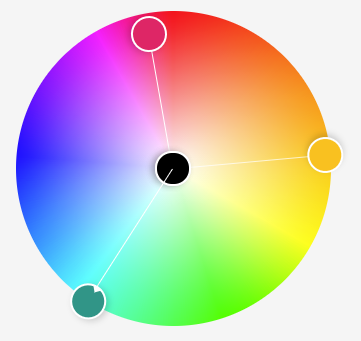
\includegraphics[width=0.35\textwidth]{../png/colors/app.png}
    \caption{Barevná paleta aplikace: Zvolené schema pro mou aplikaci} \label{picture:colors:app}
\end{figure}

\paragraph{Barvy a idempotence akce.} Jelikož mám vybrané dvě akcentní barvy, musel jsem se rohodnout, kde budu kterou z nich používat. Co se týká zobrazování, je vše poměrně jasné: k základní barvě se volně váže doplňkově-akcentní růžová, a čistě akcentní žlutá barva je ponechána pouze pro důležité položky, které je potřeba speciálně zvýraznit. Jiné je to ale u akcí - tlačítek, odkazů apod. Zde jsem se rozhodl barvu tlačítek volit dle idempotence akce, kterou vyvolávají - tedy zda vyvolaná akce způsobuje vedlejší efekty, nebo ji lze vyvolávat stále dokola. Za vedlejší efekty v aplikaci považuji následující situace:
\begin{itemize}
    \item navigace na jinou stránku,
    \item uložení či úprava dat.
\end{itemize}
Naopak akce, které nemají vedlejší efekt, jsou všechny ty, které neukládají žádná data ani nemění navigaci, mohou ale měnit aktuální zobrazení stránky, tedy například něco otevřít, skrýt, přesunout, avšak vždy tak, že se jedná o akci pouze na jednom klientu a zůstávají na jedné stránce. Na obrázcích \ref{picture:colors:time_tracker} a \ref{picture:colors:task_fab} je vidět použití jak idempotentních, tak non-idempotentních akcí: tlačítka \emph{storno} a hlavní akční tlačítko pouze skrývají dialog, respektive rozevírají menu, kdežto ostatních tlačítka a volby vždy buďto odesílají data, nebo přecházejí na novou stránku.

\begin{figure}[]
    
\includegraphics[width=0.6\textwidth]{../png/app/colors_time_tracker.png}
    \caption{Barvy znázorňující idempotenci akcí: Dialog běžícího času} \label{picture:colors:time_tracker}
\end{figure}
\begin{figure}[]
    
\includegraphics[width=0.3\textwidth]{../png/app/colors_tasks.png}
    \caption{Barvy znázorňující idempotenci akcí: Tlačítko tvorby úkolu} \label{picture:colors:task_fab}
\end{figure}

